\todo{Das muss noch woanders hin. oder raus}\\
Das \gls{CAP} Theorem, veranschaulicht in \autoref{fig:cap}, besagt, dass jedes System mit dem Daten über das Netzwerk gesendet werden, nur zwei von den drei möglichen Eigenschaften, Konsistenz, Verfügbarkeit und Partitionstoleranz, garantieren kann.
Konsitzenz der gespeicherten Daten bedeutet, es muss sichergestellt werden dass nach Abschluss der Transaktion auch alle Replikate des manipulierten Datensatzes aktualisiert werden. Der Datensatz ist in jeder Datenbank identisch.
%
\begin{figure}[H]
  \centering
  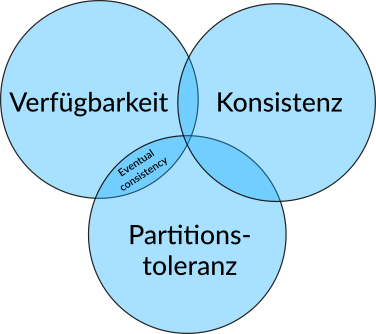
\includegraphics[width=0.6\textwidth]{cap}
  \grayRule
  \caption{Das CAP Theorem}
  \label{fig:cap}
\end{figure}
%
Das System ist besitzt eine hohe Verfügbarkeit wenn alle Anfragen an das System stets beantwortet werden. Die Verfügbarkeit ist gering, wenn die Antwortzeiten des Systems lang sind.
Partitionstoleranz ist gleichzusetzen mit Ausfalltoleranz. Die Datenbank kann auf mehreren Servern verteilt sein. Trotzdem ein Server oder eine Partition ausfällt, kann das System weiterhin funktionieren.\\
Eventual Consistency kommt häufig bei verteilten Datenbanken zur Anwendung und stellt die Konsitenz der Daten nach einem gewissen Zeitfenster sicher (vgl. ~\cite{couchDB} S. 11 ff.). 
% Wenn Verfügbarkeit Priorität hat, können wir Clients die Daten zunächst auf einen Knoten schreiben lassen, ohne darauf zu warten, dass die anderen Knoten synchronisiert werden.
% Wenn die Datenbank weiß, wie sie mit dieser Situation umzugehen hat, sind die Daten irgendwann „letztendlich konsistent“ — allerdings unter Aufgabe der Hochverfügbarkeit der Daten.
% Für viele Anwendungen ist das ein erstaunlich guter Kompromiss.